\documentclass[a4paper,papersize,dvipdfmx]{jsarticle}
\usepackage{ascmac}
\usepackage{mathtools, amssymb,bm}
\usepackage{comment}
\usepackage[hiresbb]{graphicx}
\usepackage{tcolorbox,color}
\usepackage{here}
\tcbuselibrary{raster,skins,breakable}

\newcommand{\pic}[1]{\begin{center} \includegraphics[width=1.0\linewidth,clip]{#1} \end{center}}   %写真用
\newcommand{\pict}[2]{\begin{center} \includegraphics[width= {#2} cm]{#1} \end{center}}   %写真用
\newcommand{\redunderline}[1]{\textcolor{red}{\underline{¥textcolor{black}{#1}}}}   %赤いアンダーライン
\newcommand{\mon}[1]{\item[({#1})] \ }
\newcommand{\ctext}[1]{\raise0.2ex\hbox{\textcircled{\scriptsize{#1}}}}%文字を丸囲みする(2桁の数字までならいける)

% 画像を貼る時はjpgかjpegで、pngはうまくいかないっぽい

%\itemを四角で囲った数字にする場合は以下のコメントアウトを消す
%\renewcommand{\labelenumi}{\textbf{\framebox[1.5zw]{\theenumi}}}


%enumerateの2階層めのカウンタを1,2,3, にする時は以下のコメントアウトを消す
\renewcommand{\theenumii}{\arabic{enumii}}

%enumerateのカウンタについては以下を参照
% http://www3.otani.ac.jp/fkdsemi/pLaTeX_manual/kajyo.html


%enumerateの番号の出力形式を変更するには、カウンタの値を出力する命令を定義し直す。
%レベル	カウンタ	出力する命令	デフォルトの出力
%1	enumi	¥theenumi	アラビア数字(1,2,3,・・・)
%2	enumii	¥theenumii	小文字のアルファベット(a,b,c,・・・)
%3	enumiii	¥theenumiii	小文字のローマ数字(小文字のローマ数字(\UTF{2170},\UTF{2171},\UTF{2172},・・・)
%4	enumiv	¥theenumiv	大文字のアルファベット(A,B,C,・・・)
%例:¥enumiカウンタを大文字のローマ数字で出力する設定
% ¥renewcommand{¥theenumi}{¥Roman{enumi}}

% 番号の出力形式
%命令	出力形式
%¥arabic	アラビア数字(1、2、3、・・・)
%¥roman	ローマ数字(\UTF{2170}、\UTF{2171}、\UTF{2172}、・・・)
%¥Roman	ローマ数字(\UTF{2160}、\UTF{2161}、\UTF{2162}、・・・)
%¥alph	アルファベット(a、b、c、・・・)
%¥Alph	アルファベット(A、B、C、・・・)




\begin{document}

\title{実習レポート 分析化学教室}
\author{10191043 鈴木健一}
%作成日を入れる場合は消す
\date{}
\maketitle

%以下の3つからフォントサイズを選択するとよい
%\footnotesize
\small
%\normalsize


\section*{実験 l-1 HPLCの基礎}
\begin{flushright}
実験日 : 2019/6/12

実習班 : 8班
\end{flushright}

\subsection*{目的}
ODSカラムを用いた逆相分離を行う。逆相の考え方を理解するとともに、HPLCで用いられる各種パラメーターの算出方法、分離に影響を及ぼす諸因子について考察する。

\subsection*{実験方法}
実習書に従って行った。

\subsection*{HPLC条件}
\begin{itemize}
\item 試料 : 各 0.5 $\rm \mu M$ パラベン5種混合資料
\item 注入量 : 5 $\rm \mu L$
\item HPLC装置
\item Pump : JASCOPUー980
\item Detector : JASCOUVー970
\item Integrator : JASCO807ーIT
\item 固定相 : GLサイエンス Inert Sustain C18 (150 mm x 4.6mm i.d., 5$\rm \mu m$)
\item 移動相 : $\rm MeOH-H_2O$系溶媒 (60:40, 70:30, 80:20, v/v)
\item 流速 : 1.0mL/min
\item 検出波長 : 254nm
\item チャートスビード : 5mm/min程度。ただし、MeOH-H20(60:40,v/v)を用いる場合には 2mm/minでよい。
\item ATTENUATION : 1024程度

\end{itemize}
\subsection*{結果}
クロマトグラムは代表者の物を参照

\subsubsection*{MeOH : $\rm H_2O$ = 60 : 40}

\begin{itemize}
\item チャートスピード : 5 mm/min
\item ATTENUATION : 512

\begin{table}[H]
\begin{center}
\begin{tabular}{|c|c|c|c|c|c|c|}
\hline
&  $t_R(mm)$ & $t_R(min)$ & $W_{1/2}(mm)$ & $W_{1/2}(min)$ & $k^\prime$   & N    \\ \hline
$\rm H_2O$      & 8.46      & 1.692          &                 & 0.00 & 0.00  &  \\ \hline
C1       & 19.84     & 3.967          & 0.9             & 0.18 & 1.34  & 2690.85  \\ \hline
C2       & 28.63     & 5.725          & 1.0             & 0.20 & 2.38  & 4539.42  \\ \hline
C3       & 46.13     & 9.225          & 1.2             & 0.24 & 4.45  & 8185.03  \\ \hline
C4       & 79.96     & 15.992         & 2.0             & 0.40 & 8.45  & 8855.14  \\ \hline
C5       & 144.50    & 28.900         & 3.5             & 0.70 & 16.08 & 9442.99  \\ \hline
\end{tabular}
\end{center}
\end{table}

\begin{table}[H]
\begin{center}
\begin{tabular}{|c|c|c|}
\hline
& α     & Rs         \\ \hline
C1-C2 & 1.77 & 5.44  \\ \hline
C2-C3 & 1.87 & 9.36  \\ \hline
C3-C4 & 1.90 & 12.44 \\ \hline
C4-C5 & 1.90 & 13.81 \\ \hline
\end{tabular}
\end{center}
\end{table}

\end{itemize}
\subsubsection*{MeOH : $\rm H_2O$ = 70 : 30}

\begin{itemize}
\item チャートスピード : 10 mm/min
\item ATTENUATION : 512

\begin{table}[H]
\begin{center}
\begin{tabular}{|c|c|c|c|c|c|c|}
\hline
&  $t_R(mm)$ & $t_R(min)$ & $W_{1/2}(mm)$ & $W_{1/2}(min)$ & $k^\prime$   & N    \\ \hline
$\rm H_2O$                & 16.92    & 1.692     &                & 0.00            & 0.00 &  \\ \hline
C1                 & 27.67    & 2.767     & 1.0            & 0.10            & 0.64 & 4241.58  \\ \hline
C2                 & 34.33    & 3.433     & 1.0            & 0.10            & 1.03 & 6529.16  \\ \hline
C3                 & 46.08    & 4.608     & 1.2            & 0.12            & 1.72 & 8169.06  \\ \hline
C4                 & 66.08    & 6.608     & 2.0            & 0.20            & 2.91 & 6047.69  \\ \hline
C5                 & 99.67    & 9.967     & 2.6            & 0.26            & 4.89 & 8141.27  \\ \hline
\end{tabular}
\end{center}
\end{table}

\begin{table}[H]
\begin{center}
\begin{tabular}{|c|c|c|}
\hline
& α     & Rs       \\ \hline
C1-C2 & 1.62 & 3.92 \\ \hline
C2-C3 & 1.67 & 6.28 \\ \hline
C3-C4 & 1.69 & 7.35 \\ \hline
C4-C5 & 1.68 & 8.59 \\ \hline
\end{tabular}
\end{center}
\end{table}


\end{itemize}
\subsubsection*{MeOH : $\rm H_2O$ = 80 : 20}

\begin{itemize}
\item チャートスピード : 20 mm/min
\item ATTENUATION : 1024

\begin{table}[H]
\begin{center}
\begin{tabular}{|c|c|c|c|c|c|c|}
\hline
&  $t_R(mm)$ & $t_R(min)$ & $W_{1/2}(mm)$ & $W_{1/2}(min)$ & $k^\prime$   & N    \\ \hline
$\rm H_2O$      & 33.84     & 1.692          &                 & 0.00 & 0.00 &         \\ \hline
C1       & 45.16     & 2.258          & 1.9             & 0.10 & 0.33 & 3129.76 \\ \hline
C2       & 50.66     & 2.533          & 2.0             & 0.10 & 0.50 & 3554.51 \\ \hline
C3       & 59.66     & 2.983          & 2.0             & 0.10 & 0.76 & 4929.65 \\ \hline
C4       & 73.16     & 3.658          & 2.4             & 0.12 & 1.16 & 5147.95 \\ \hline
C5       & 93.16     & 4.658          & 3.0             & 0.15 & 1.75 & 5342.27 \\ \hline
\end{tabular}
\end{center}
\end{table}


\begin{table}[H]
\begin{center}
\begin{tabular}{|c|c|c|c|}
\hline
& α    & Rs   &  \\ \hline
C1-C2 & 1.49 & 1.66 &  \\ \hline
C2-C3 & 1.54 & 2.65 &  \\ \hline
C3-C4 & 1.52 & 3.61 &  \\ \hline
C4-C5 & 1.51 & 4.36 &  \\ \hline
\end{tabular}
\end{center}
\end{table}

\pict{imgs/kp.png}{10}
\pict{imgs/log_kp.png}{10}

\end{itemize}
\subsection*{考察}

\begin{tcolorbox}[colback=white,colbacktitle=black!10!white,coltitle=black,title={1}]
移動層の極性を変化させることによってパラペンの保持係数はどのように変化するか。
\end{tcolorbox}

グラフより、MeOHの濃度が高い、つまり極性が小さくなるほど保持係数も小さくなる。また、$\log k^\prime$と濃度グラフを書くと線形性がみられることがわかる。

\begin{tcolorbox}[colback=white,colbacktitle=black!10!white,coltitle=black,title={2}]
各パラメーターがどのような状態になれば、分離が良好な状態になるか。
\end{tcolorbox}

保持係数$k^\prime$はピークの広がりを示す指標である。$k^\prime$が小さすぎるとカラムでの分離が十分できておらず、大きすぎるとピークが広がりすぎるため、$1 \leq k^\prime \leq 10$が最適な範囲とされる。
分離係数$\alpha$はピーク同士の離れ具合を表すので$\alpha$が大きいほど分離が良い。
分離度$Rs$はピークの広がり具合を加味した上での離れ具合を表しており、$Rs > 1.5$であればピークは完全に分離しているとされる。

\begin{tcolorbox}[colback=white,colbacktitle=black!10!white,coltitle=black,title={3}]
パラペンの分離を速く、かつ良好に行うにはどうしたら良いのか。
\end{tcolorbox}

移動層の極性を適切に設定することで分離が適切に行われる。

\subsection*{課題}
\begin{tcolorbox}[colback=white,colbacktitle=black!10!white,coltitle=black]
逆層分離の原理を充填剤の構造と本実験の結果に言及しながら説明する。
\end{tcolorbox}

逆層分離は低極性の充填剤をカラムに詰めてその中を移動層が流すことで低極性の物質が吸着し、高極性のものから順に溶出させる分離法である。本実験で用いたODSはシリカゲルの表面に疎水性のオクタデシルシリル基がついたものであり、炭素数が多いパラベンを強く吸着する。

\subsection*{感想}
研究室ごとに課題が出されるため、書くべきレポートが多すぎて困ってます。

\newpage

\section*{実験 l-2 HPLCによる未知試料中DNS-アミノ酸の定性・定量分析}
\begin{flushright}
実験日 : 2019/6/13

実習班 : 8班
\end{flushright}

\subsection*{目的}
ダンシルクロリドで誘導体化したアミノ酸混合試料を、逆相HPLCにより分離同定し、さらにその濃度を定量する。定量の際には、絶対検量線法と内標準法という2つの方法を用いてDNS-アミノ酸の検量線を作成し、未知試料中の各DNS-アミノ酸濃度を決定する。

\subsection*{実験方法}
実習書に従って行った。

\subsection*{HPLC条件}
\begin{itemize}
\item 固定相 : GLサイエンス InertSustain C18 (150mm x 4.6mm i.d., 5$\rm \mu m$)
\item 移動相 : $\rm MeOH : H_2O$ = 40 : 60, trifluoroacetic acid (TFA) 0.1%
\item 流速 : 0.8mL/min
\item 検出波長 : 340nm
\item チャートスピード : 2mm/min
\item ATTENUATION : 16程度
\item 試料注入量 : $5 \  \rm \mu L$

\end{itemize}
\subsection*{結果}

クロマトグラムはレポート末に添付してます。

\begin{table}[H]
\begin{center}
\begin{tabular}{|c|c|c|c|c|c|}
\hline
DNS-アミノ酸濃度(mM) & 0     & 0.2   & 0.4   & 0.6   & 0.8   \\ \hline
Ser            & 0.000 & 4.542 & 4.583 & 4.575 & 4.592 \\ \hline
Asp            & 0.000 & 5.033 & 5.067 & 5.067 & 5.083 \\ \hline
Gly            & 5.517 & 5.550 & 5.583 & 5.583 & 5.600 \\ \hline
Thr            & 0.000 & 6.317 & 6.367 & 6.367 & 6.383 \\ \hline
Ala            & 0.000 & 7.500 & 7.542 & 7.550 & 7.567 \\ \hline
\end{tabular}
\caption{保持時間}
\end{center}
\end{table}

\begin{table}[H]
\begin{center}
\begin{tabular}{|c|c|c|c|c|c|}
\hline
DNS-アミノ酸濃度(mM) & 0    & 0.2  & 0.4  & 0.6  & 0.8  \\ \hline
Ser            &      & 1461 & 3029 & 4673 & 6448 \\ \hline
Asp            &      & 1317 & 2704 & 4191 & 5649 \\ \hline
Gly            & 3071 & 3288 & 3079 & 3054 & 3057 \\ \hline
Thr            &      & 1128 & 2349 & 3710 & 4956 \\ \hline
Ala            &      & 1070 & 2234 & 3517 & 4742 \\ \hline
\end{tabular}
\caption{ピーク高さ}
\end{center}
\end{table}


\begin{table}[H]
\begin{center}
\begin{tabular}{|c|c|c|c|c|c|}
\hline
DNS-アミノ酸濃度(mM)  & 0.2   & 0.4   & 0.6   & 0.8   \\ \hline
Ser              & 0.444 & 0.984 & 1.530 & 2.109 \\ \hline
Asp              & 0.401 & 0.878 & 1.372 & 1.848 \\ \hline
Thr              & 0.343 & 0.763 & 1.215 & 1.621 \\ \hline
Ala              & 0.325 & 0.726 & 1.152 & 1.551 \\ \hline
\end{tabular}
\caption{内標準物質(DNS-Gly)とのピーク高さ比}
\end{center}
\end{table}

\pict{imgs/1-2-1.png}{14}
\pict{imgs/1-2-2.png}{14}

未知試料からは以下のようなアミノ酸が検出された。またその結果と上のグラフで得た検量線をもとに算出したアミノ酸の濃度は以下の通りである。



\begin{table}[H]
\begin{center}
\begin{tabular}{|c|c|c|c|c|}
\hline
アミノ酸 & ピーク高さ [a.u.] & 算出された濃度(mM) & 実際の濃度(mM) & 誤差(\%) \\ \hline
Ser  & 4862  & 0.770 & 0.770 & 0.00 \\ \hline
Asp  & 1971  & 0.359 & 0.330 & 8.79 \\ \hline
Gly  & 3078  & 2.520 & 2.000 & 26.0 \\ \hline
Thr  & 2773  & 0.596 & 0.550 & 8.36  \\ \hline
\end{tabular}
\caption{絶対検量線法}
\end{center}
\end{table}

\begin{table}[H]
\begin{center}
\begin{tabular}{|c|c|c|c|c|}
\hline
アミノ酸 & ピーク高さ比 & 算出された濃度 & 実際の濃度(mM) & 誤差(\%) \\ \hline
Ser  & 1.580  & 0.767 & 0.770 & 0.00 \\ \hline
Asp  & 0.640  & 0.362 & 0.330 & 8.79  \\ \hline
Gly  & 1.000  & 2.511 & 2.000 & 25.6 \\ \hline
Thr  & 0.901  & 0.597 & 0.550 & 8.55 \\ \hline
\end{tabular}
\caption{内標準法}
\end{center}
\end{table}


\subsection*{考察}
絶対検量線法と内標準法でそれぞれ算出された濃度に大きな差はなかった。また、グラフの決定係数も0.99を超えているので十分な直線性が得られたと言える。また、Glyのみ算出された濃度と実測値に誤差があったが、これは混合溶液をHPLCに入れる際に$5\rm \mu L$よりも多く入れたことが原因だと推測される。

\subsection*{課題}

\begin{tcolorbox}[colback=white,colbacktitle=black!10!white,coltitle=black,title={1}]
絶対検量線法による定量の際に気をつけなければならない点を挙げる。
\end{tcolorbox}

ピーク高さが濃度だけでなく、HPLCに入れた試料の量にも比例するので入れる量を正確に測る必要がある。

\begin{tcolorbox}[colback=white,colbacktitle=black!10!white,coltitle=black,title={2}]
内標準法による定量の際に内標準物質としてどのような化合物を選択しなければならないか。
\end{tcolorbox}

試料と反応せず、かつ他の物質とピークが完全に分離している必要がある。

\begin{tcolorbox}[colback=white,colbacktitle=black!10!white,coltitle=black,title={3}]
標準添加法について簡潔に説明する。
\end{tcolorbox}

未知試料中に含まれている物質を一定の濃度ずつ添加していき、ピーク高さを縦軸に、添加した濃度を横軸にして検量線を作成すると、濃度が負になる領域で検量線が横軸と交わる。その点と原点の距離を求める成分の濃度として得ることができるという手法が標準添加法である。


\subsection*{感想}
1日でレポートを書き上げるのは大変ですが、だからと言って毎日コツコツやるのも大変なものです。\newpage

\section*{実験 ll-1 吸光法}

\begin{flushright}
実験日 : 2019/6/11

実習班 : 8班
\end{flushright}

\subsection*{目的}
吸光法について学ぶ

\subsection*{実験操作}
実習書にしたがって行った。

\subsection*{スペクトル測定条件}
測定波長 : 300 $\sim$ 700 nm
吸光度スケール : 0.000 $\sim$ 1.000

\subsection*{結果}

\subsubsection*{pH指示薬}
\begin{figure}[H]
\begin{center}
\begin{tabular}{c}

\begin{minipage}{0.22\hsize}
\begin{center}
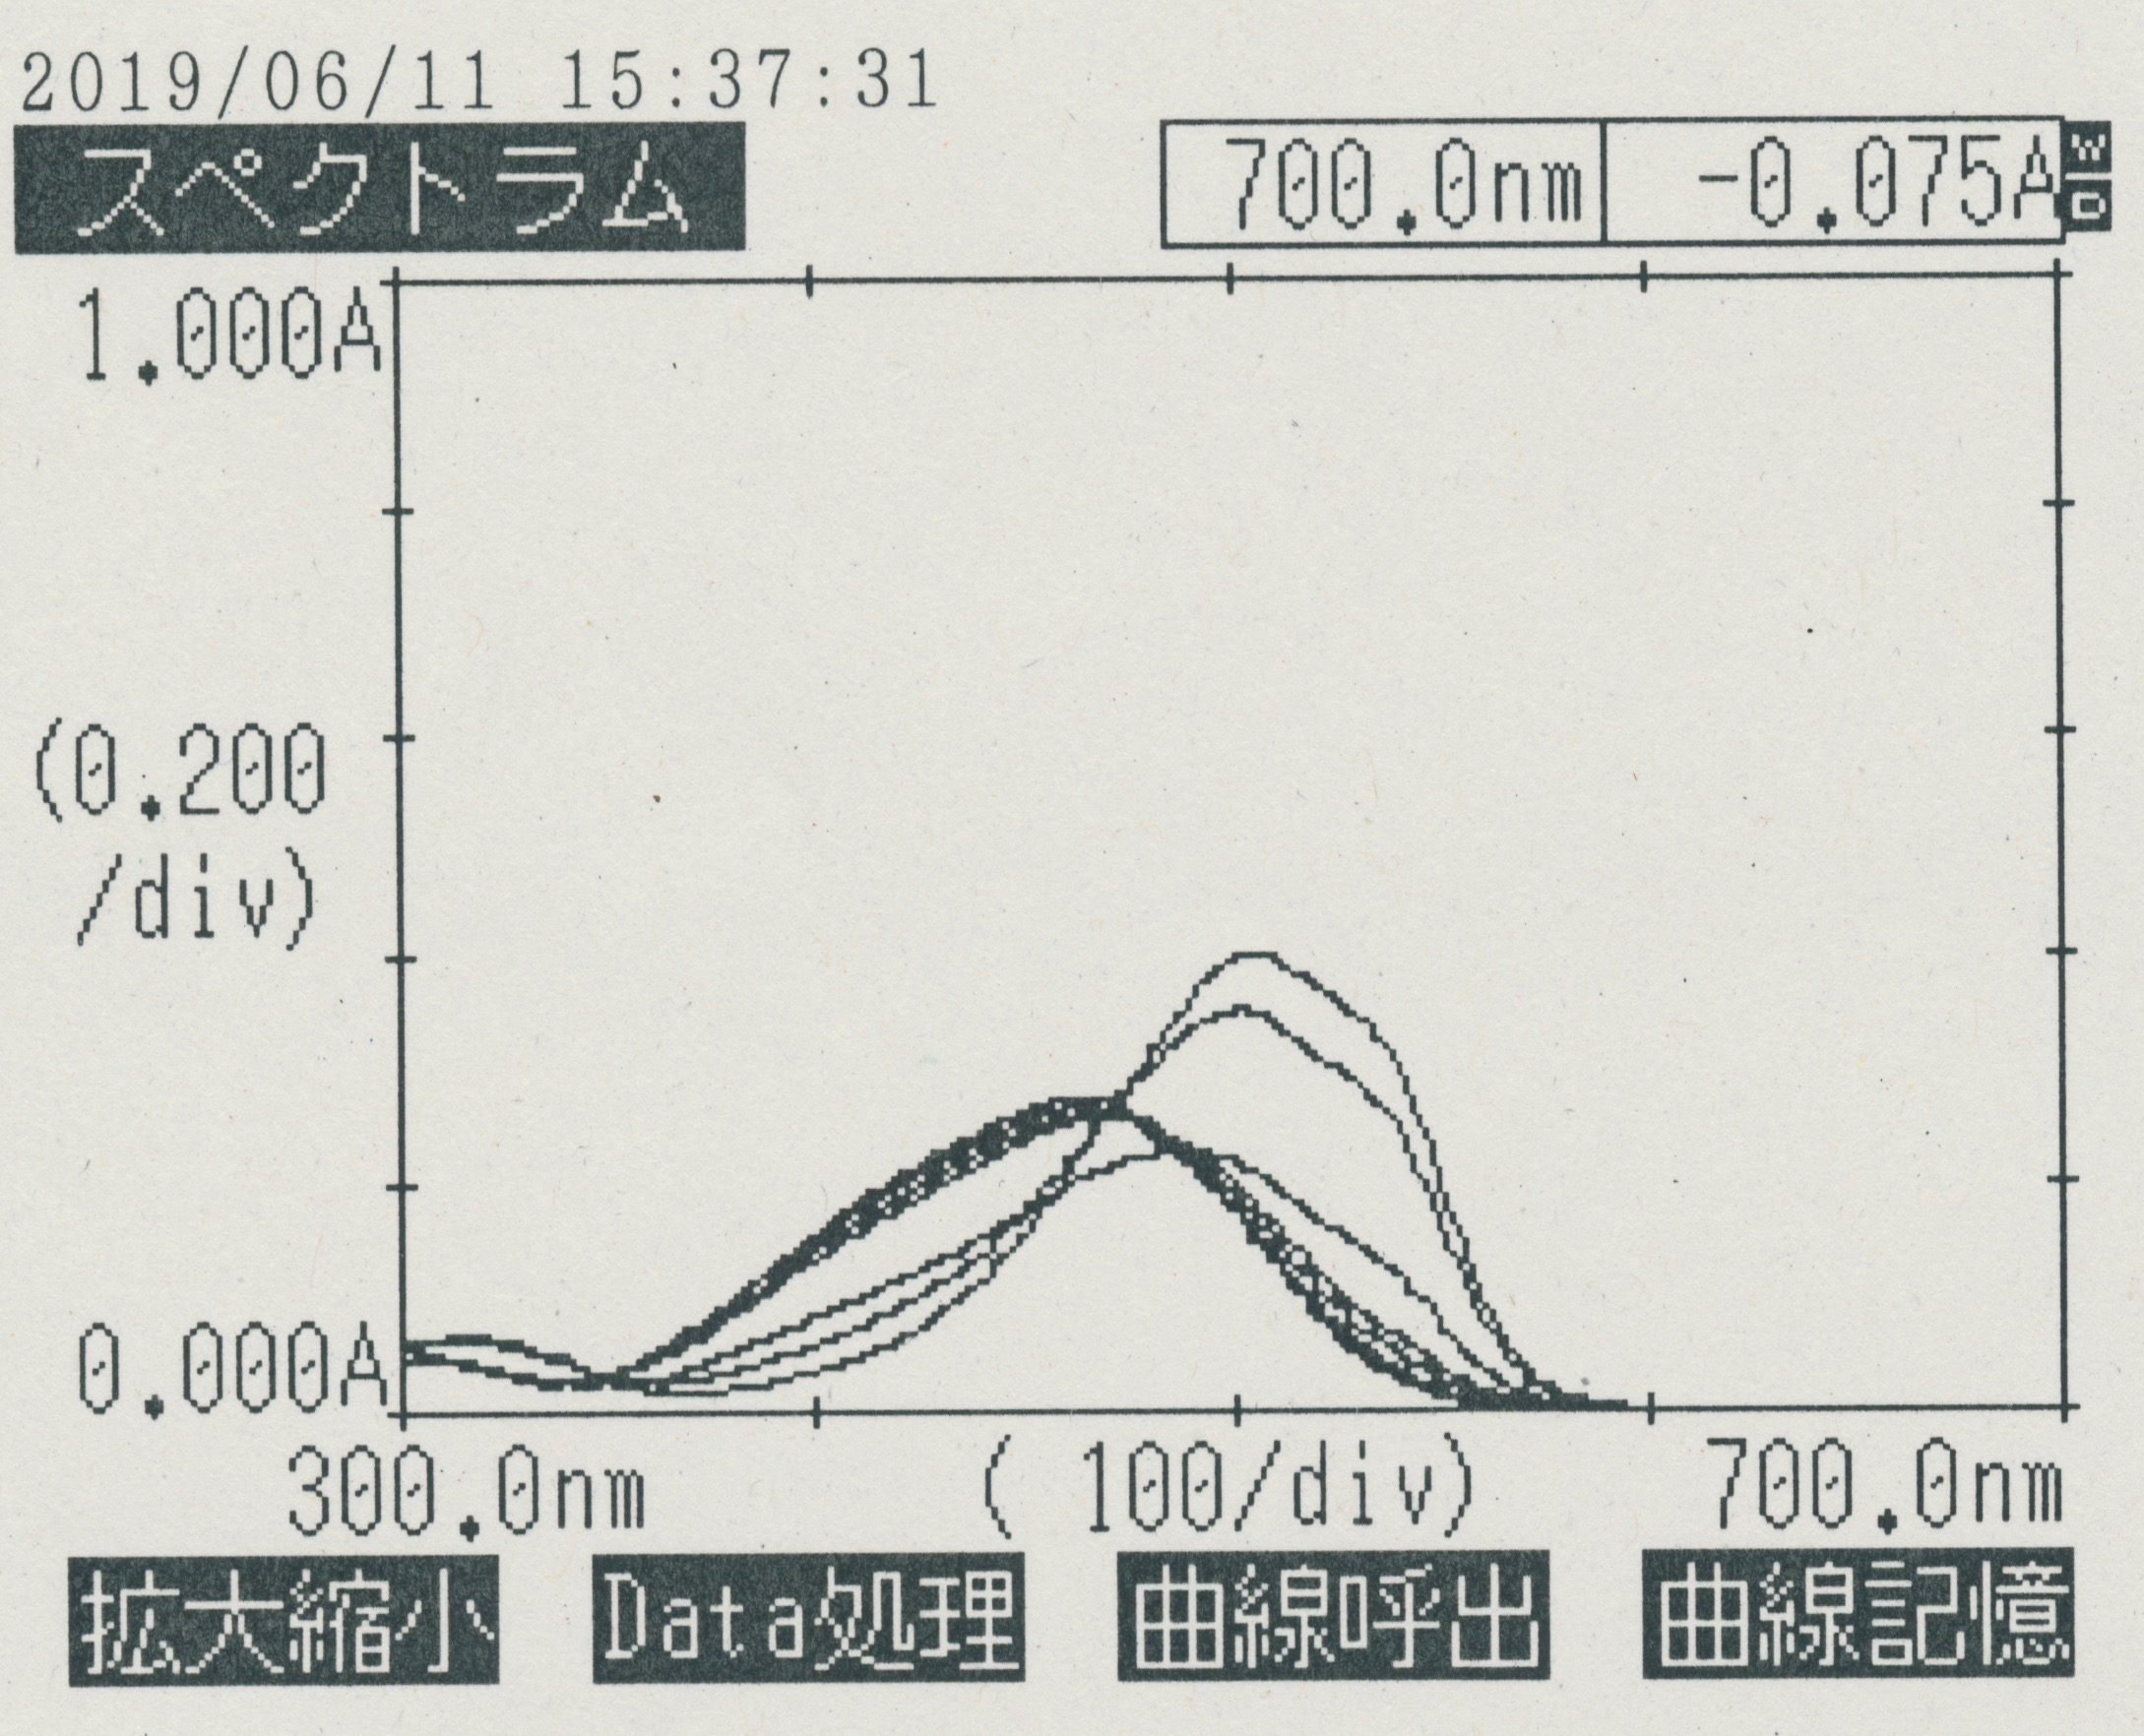
\includegraphics[clip, height=4cm]{imgs/MO.jpg}
\caption{メチルオレンジ}
\end{center}
\end{minipage}

\begin{minipage}{0.15\hsize}
\hspace{10mm}
\end{minipage}

\begin{minipage}{0.22\hsize}
\begin{center}
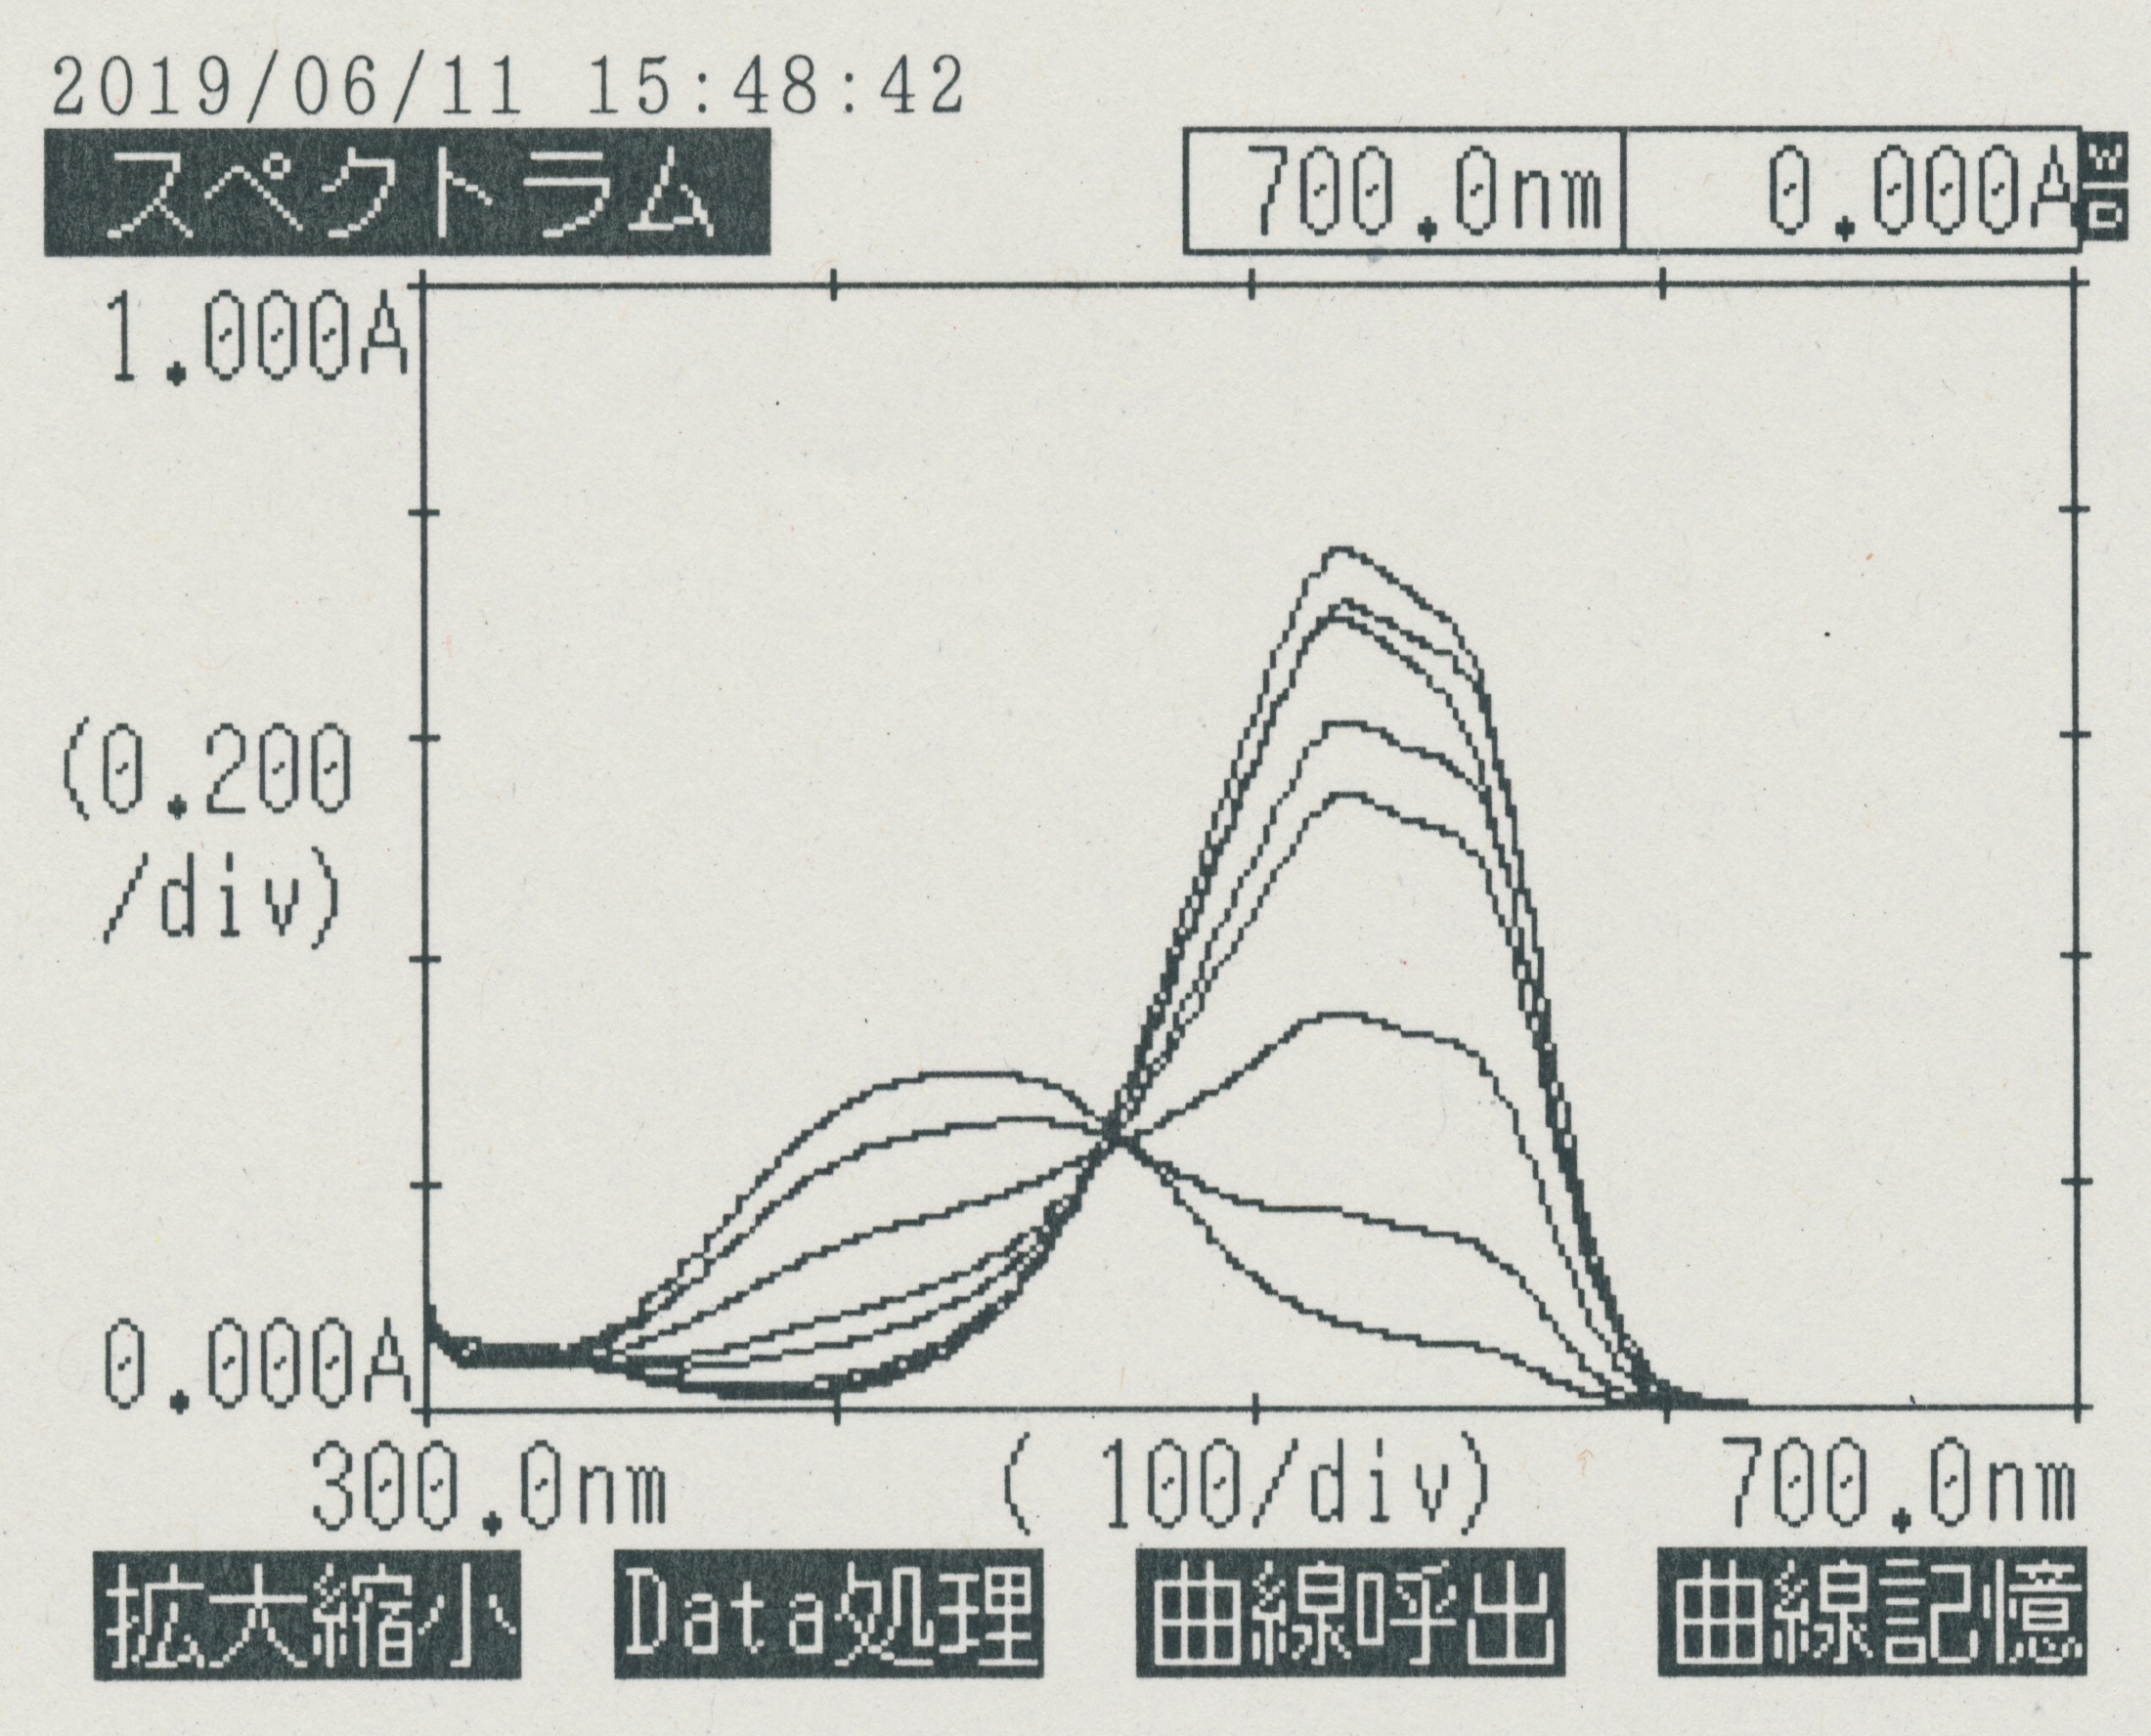
\includegraphics[clip, height=4cm]{imgs/MR.jpg}
\caption{メチルレッド}
\end{center}
\end{minipage}

\end{tabular}
\end{center}
\end{figure}

メチルオレンジとメチルレッドがpHに応じて最大吸収波長、吸光度、モル吸光係数が変化する様子を以下の表にまとめた。

\begin{table}[H]
\begin{center}
\begin{tabular}{|c|c|c|c|}
\hline
pH & $\lambda$  & Abs   & $\epsilon$     \\ \hline
2.5 & 506.000 & 0.404 & 40400 \\ \hline
3.0 & 503.000 & 0.354 & 35400 \\ \hline
3.5 & 490.000 & 0.228 & 22800 \\ \hline
4.0 & 470.000 & 0.260 & 26000 \\ \hline
4.5 & 468.000 & 0.263 & 26300 \\ \hline
5.0 & 464.000 & 0.268 & 26800 \\ \hline
5.5 & 464.000 & 0.276 & 27600 \\ \hline
6.0 & 464.000 & 0.268 & 26800 \\ \hline
\end{tabular}
\caption{メチルオレンジ}
\end{center}
\end{table}


\begin{table}[H]
\begin{center}
\begin{tabular}{|c|c|c|c|}
\hline
pH & $\lambda$  & Abs   & $\epsilon$     \\ \hline
2.5 & 522.000 & 0.701 & 70100 \\ \hline
3.0 & 524.000 & 0.763 & 76300 \\ \hline
3.5 & 524.000 & 0.716 & 71600 \\ \hline
4.0 & 524.000 & 0.612 & 61200 \\ \hline
4.5 & 524.000 & 0.546 & 54600 \\ \hline
5.0 & 522.000 & 0.353 & 35300 \\ \hline
5.5 & 446.000 & 0.257 & 25700 \\ \hline
6.0 & 434.000 & 0.300 & 30000 \\ \hline
\end{tabular}
\caption{メチルレッド}
\end{center}
\end{table}

\subsubsection*{金属錯体}

\begin{figure}[H]
\begin{center}
\begin{tabular}{c}

\begin{minipage}{0.22\hsize}
\begin{center}
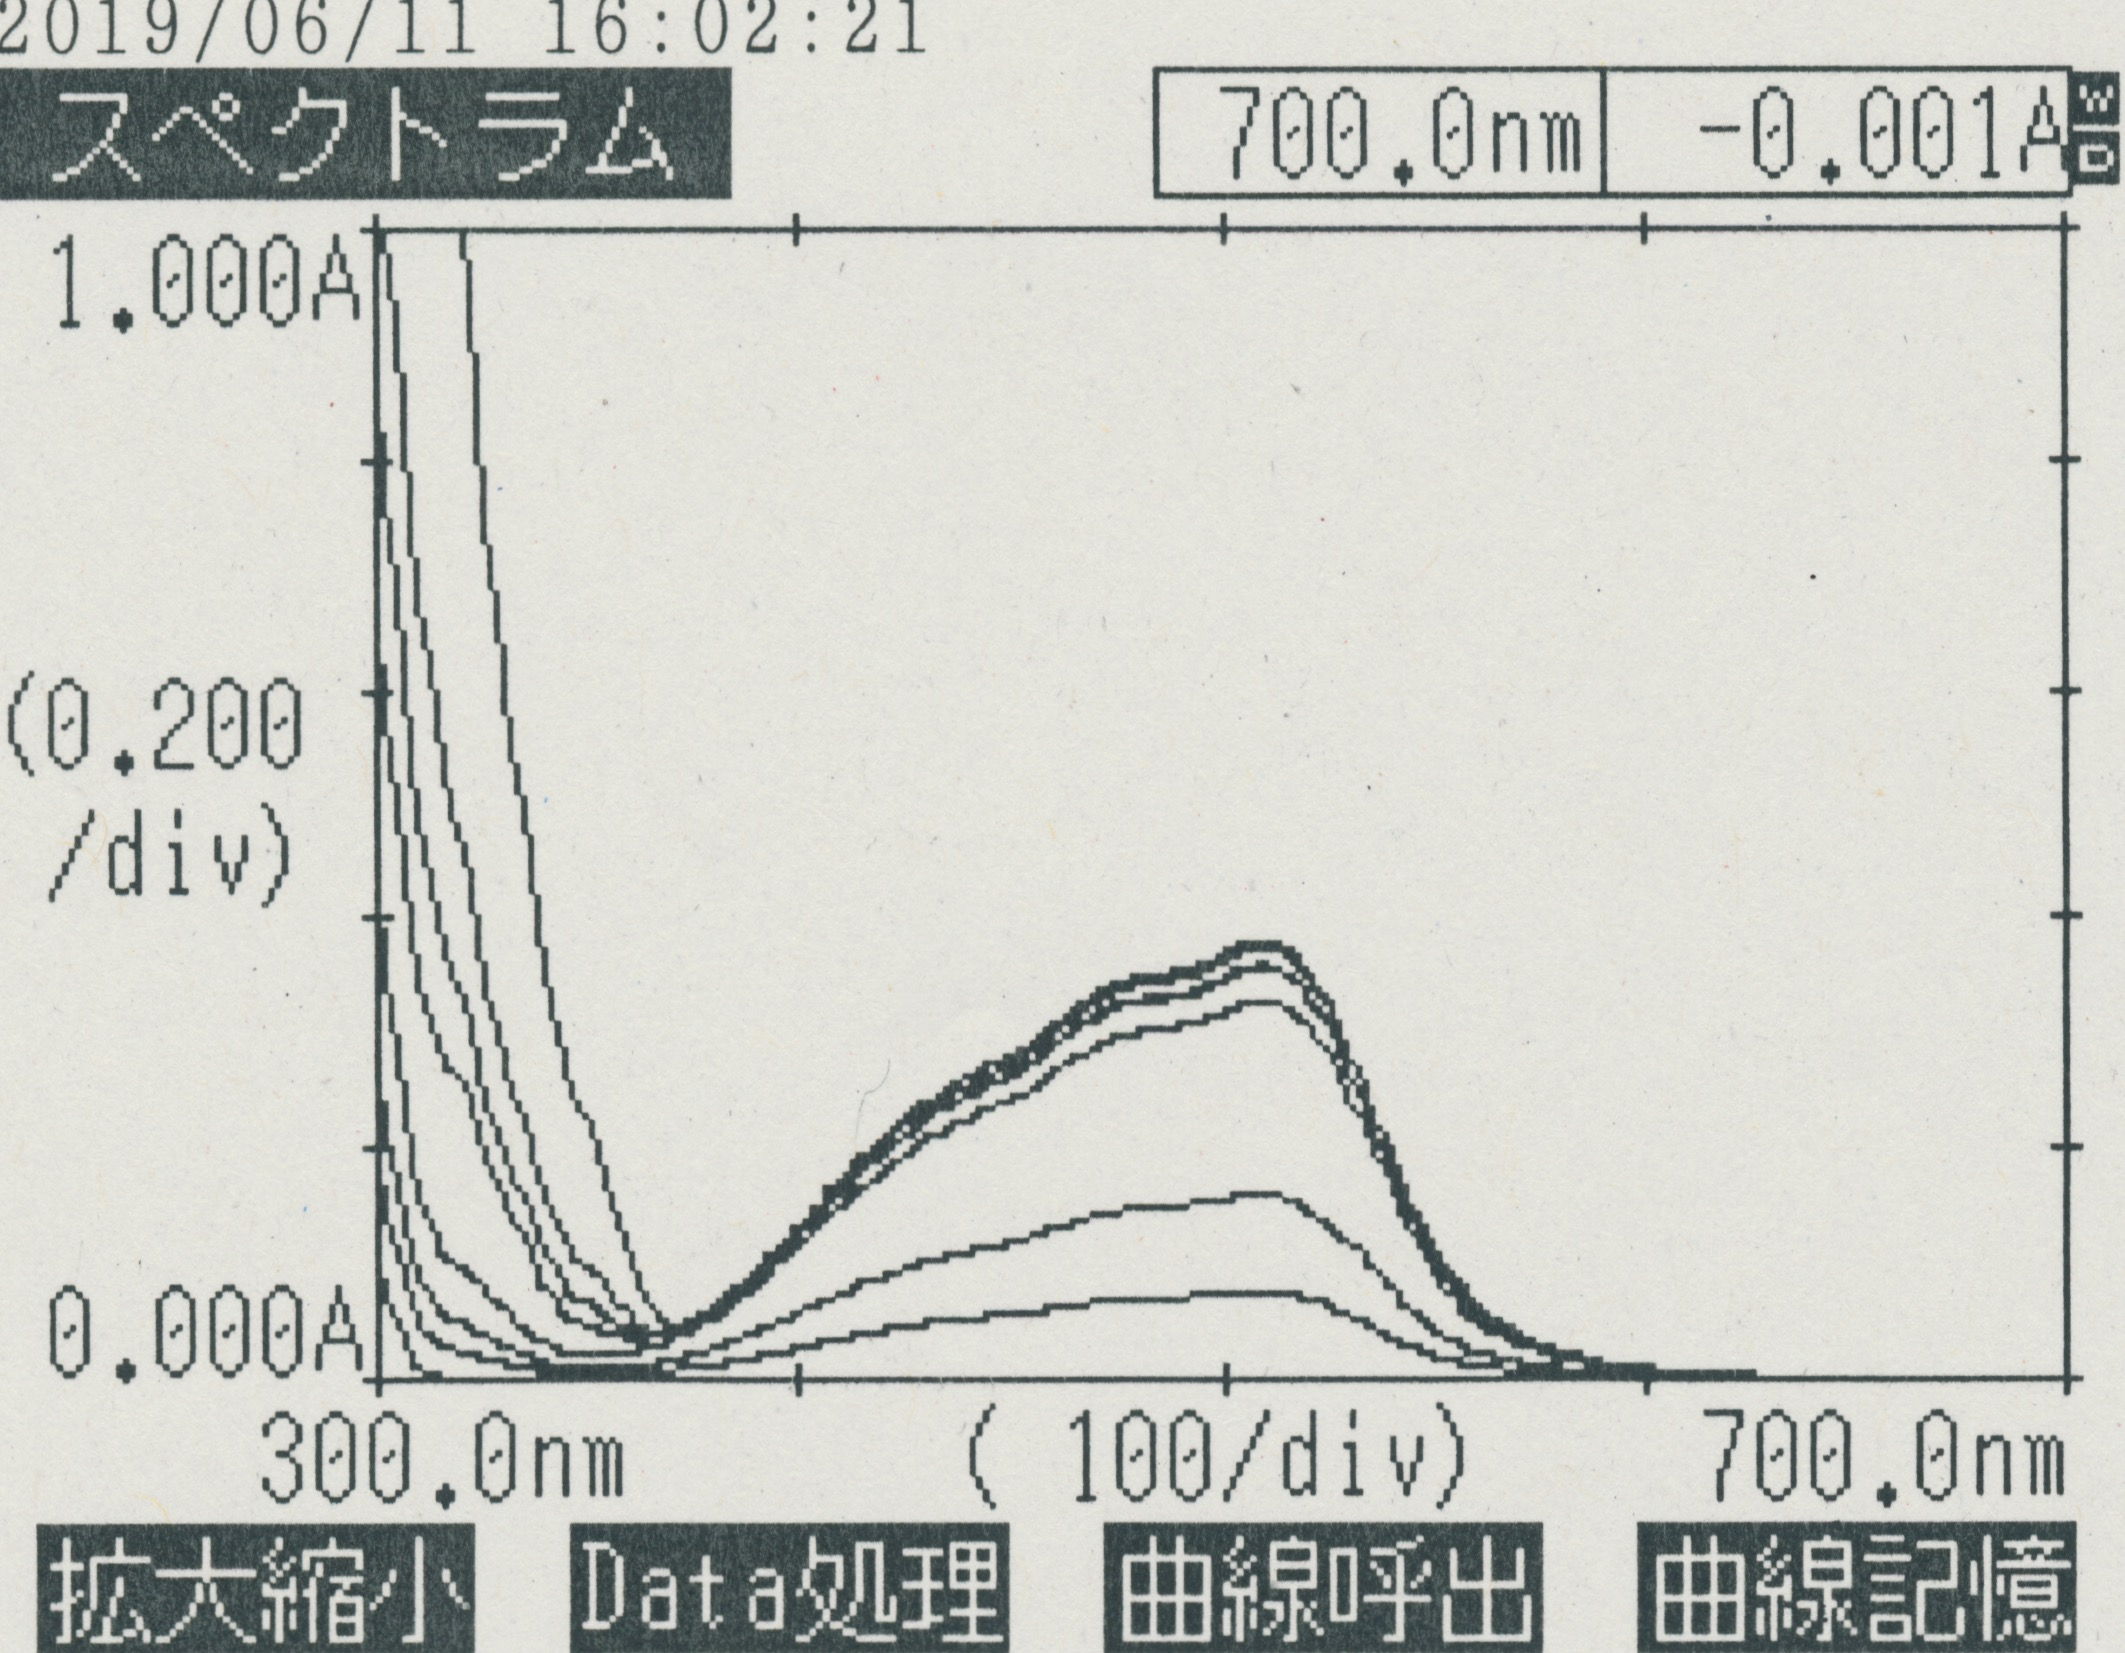
\includegraphics[clip, height=4cm]{imgs/Phe.jpg}
\caption{フェナントロリン}
\end{center}
\end{minipage}

\begin{minipage}{0.10\hsize}
\hspace{10mm}
\end{minipage}

\begin{minipage}{0.22\hsize}
\begin{center}
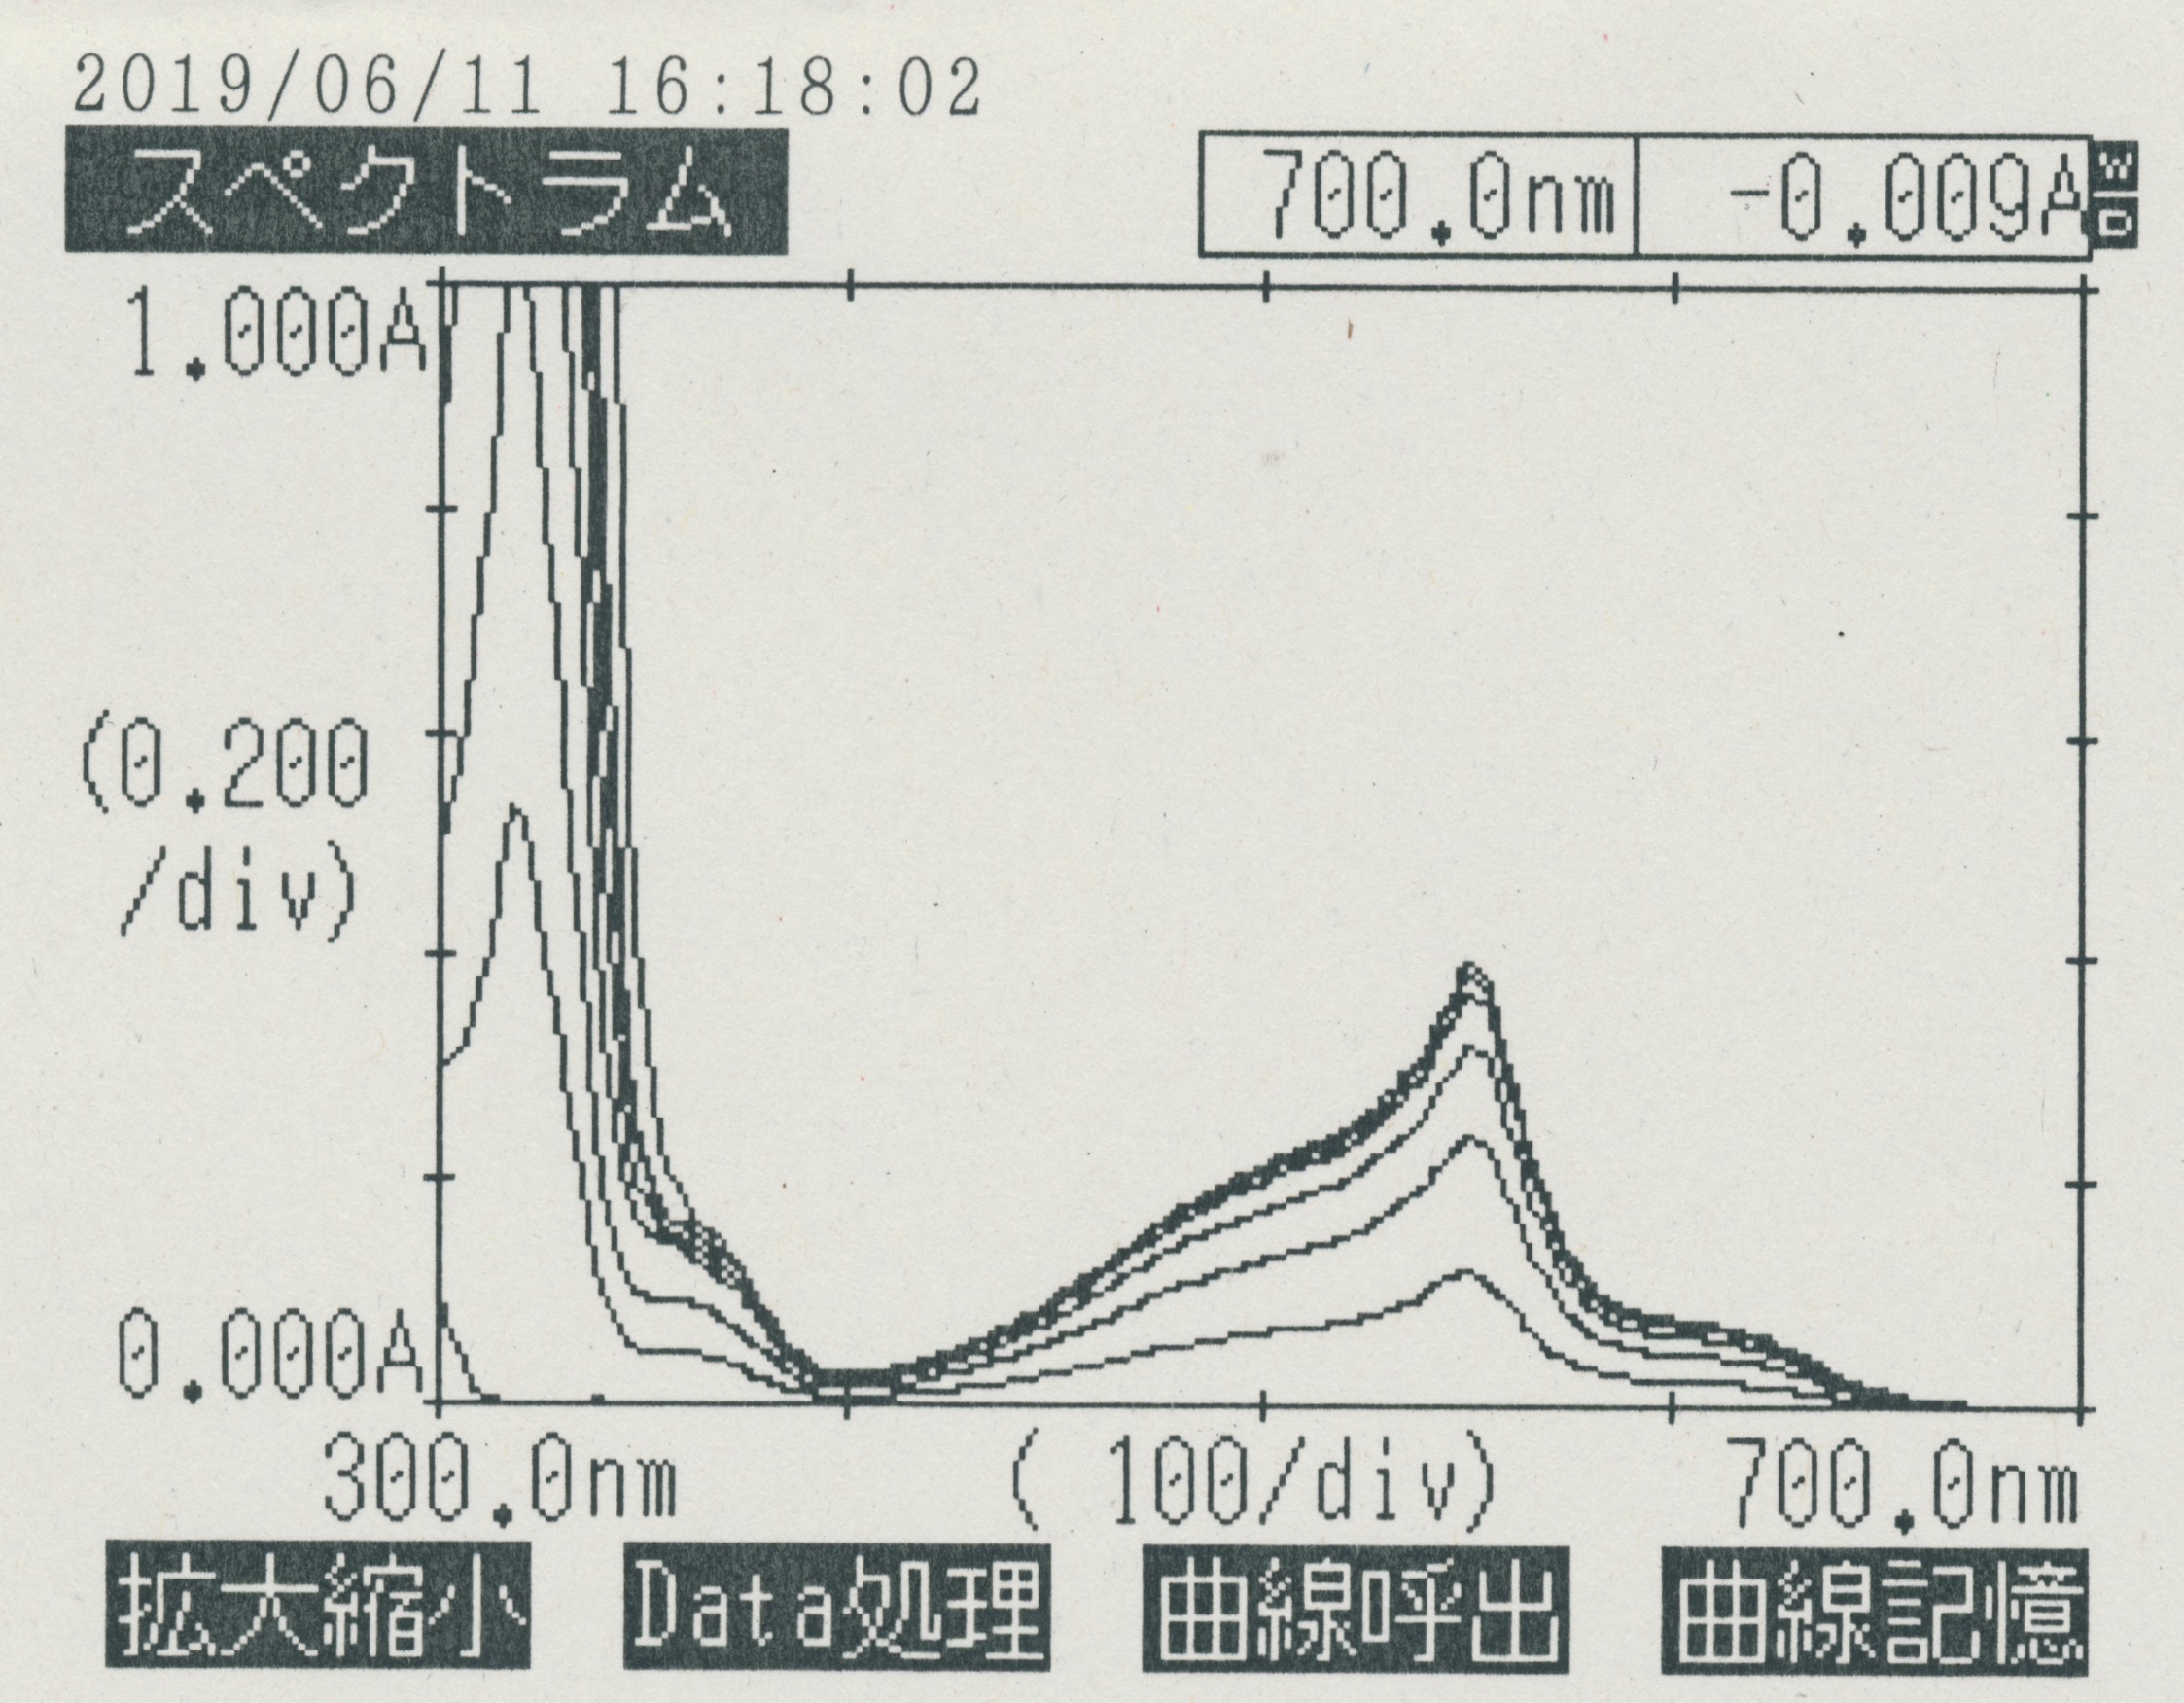
\includegraphics[clip, height=4cm]{imgs/Ter.jpg}
\caption{テルピリジン}
\end{center}
\end{minipage}

\end{tabular}
\end{center}
\end{figure}


以下の表とグラフは画像のスペクトルを元に吸光度をまとめたものである。

\begin{table}[H]
\begin{center}
\begin{tabular}{|c|c|c|}
\hline
Ligand [$\rm \mu L$] & Phenanthroline & Terpyridine \\ \hline
0               & 0.000          & 0.000       \\ \hline
50              & 0.076          & 0.120       \\ \hline
100             & 0.162          & 0.239       \\ \hline
200             & 0.329          & 0.370       \\ \hline
300             & 0.374          & 0.368       \\ \hline
400             & 0.380          & 0.395       \\ \hline
500             & 0.359          & 0.321       \\ \hline
900             & 0.357          & 0.384       \\ \hline
\end{tabular}
\end{center}
\end{table}


\pict{imgs/sp.png}{12}

フェナントロリンは3配位、テルピリジンは2配位であると考えられる。

\subsection*{考察}
今回得たスペクトラムからはMRに等吸収点が存在し、MOには存在しないような結果が得られたが、実際には逆である。

\subsection*{課題}

\subsubsection*{2-1-1}

\

\begin{tcolorbox}[colback=white,colbacktitle=black!10!white,coltitle=black,title={1}]
Lambert-Beerの法則について説明せよ
\end{tcolorbox}

吸光度は濃度が一定の場合では光が透過する長さ(光路長)に比例する。これをランベルトの法則という。
また、、一定の厚さの溶液層(一定の光路長)を通過する光の強度の減少は溶液のモル濃度に比例する。すなわち、吸光度はモル濃度に比例する。これをベールの法則という。
これらの2つの法則を合わせたものがランベルト・ベールの法則であり、以下の式が成立する。

\[A =\epsilon \cdot c \cdot l\]

溶液の吸光度は、溶液の濃度と溶液層の厚さ(セルの光路長)に比例することがわかる。

\begin{tcolorbox}[colback=white,colbacktitle=black!10!white,coltitle=black,title={2}]
pH2.5および6.0のbuffer中におけるメチルレッドとメチルオレンジの最大吸収波長、モル吸光係数を求めよ。
\end{tcolorbox}

「結果」の項にある表を参照。

\begin{tcolorbox}[colback=white,colbacktitle=black!10!white,coltitle=black,title={3}]
物質の吸収波長と色の関係をまとめ、pHによるメチルレッドとメチルオレンジの変化を説明せよ。
\end{tcolorbox}

メチルレッドpH2.5のとき、メチルレッドは緑色の光である430  $\sim$ 480 nm
の光を吸収し、メチルオレンジは青色の光である500 $\sim$ 560 nm の光を吸収する。光が反射して我々の目に見えるのは、試薬が吸収した色の補色であるため、メチルレッドとメチルオレンジはそれぞれ赤とオレンジ色に見える。

\begin{tcolorbox}[colback=white,colbacktitle=black!10!white,coltitle=black,title={4}]
等吸収点が現れる条件は何か説明せよ。
\end{tcolorbox}

物質がn通りに変化するとき、吸光度の式は以下のような線型結合な式で表される。

\[A = \Sigma_{i=1}^n \left( \ \epsilon _i \cdot c_i \cdot l \right)\]

今回の実験のように1つの物質がn通りに変化する時は、それぞれの濃度の総和は常に等しいことから、定数$C$を用いて以下の式がなりたつ。
\[\Sigma_{i=1}^n  \ c_i = C \]
これを$c_n$について整理すると
\[c_n = C - \Sigma_{i=1}^{n-1} \ c_i\]


となるので、これを吸光度の式に代入すると以下のようになる。
\[\frac{A}{l} = C \epsilon_n + \Sigma_{i=1}^{n-1}  \ c_i \left( \epsilon_i -\epsilon_n\right)\]

したがって、$c_1 \sim c_n$の濃度に関わらず吸光度が一定になる、つまり等吸収点が存在するのは以下の式が成り立つ時である。

\[\epsilon _1 = \epsilon _2 = \cdots = \epsilon _n\]

このとき$A$は一定となる。


\begin{tcolorbox}[colback=white,colbacktitle=black!10!white,coltitle=black,title={5}]
メチルレッド、メチルオレンジは等吸収点を持つか。
\end{tcolorbox}


\begin{figure}
\begin{center}
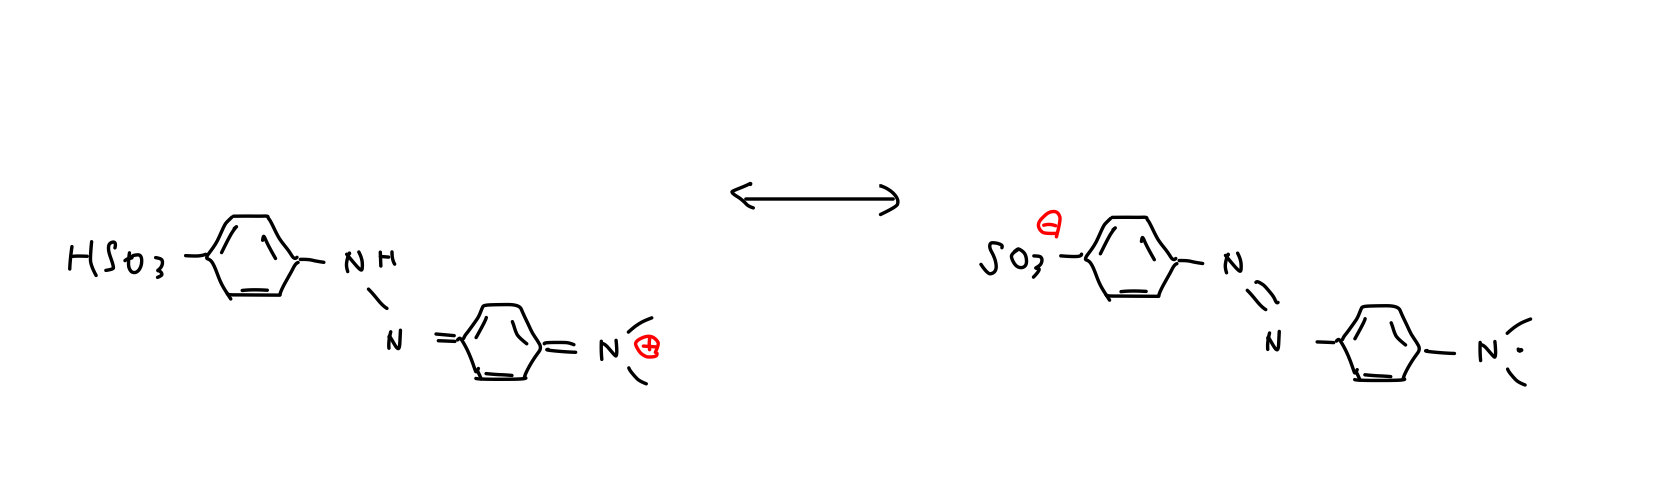
\includegraphics[clip, width=10cm]{imgs/mo.jpeg}
\caption{メチルオレンジ}
\end{center}
\end{figure}


\begin{figure}
\begin{center}
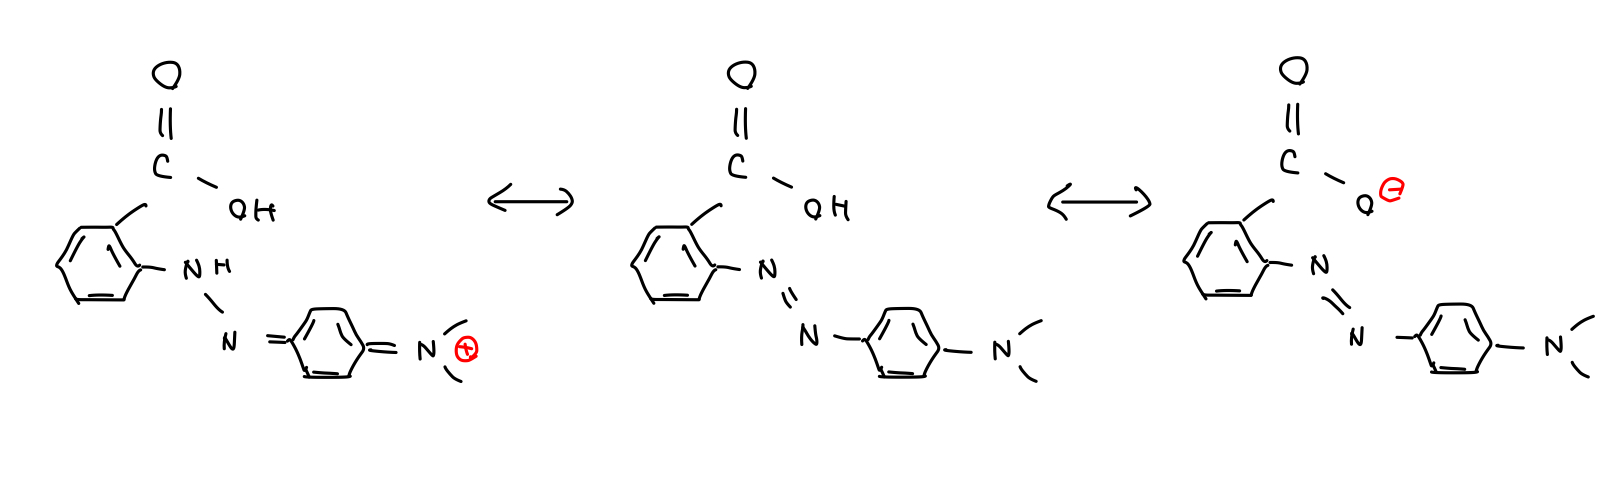
\includegraphics[clip, width=14cm]{imgs/mr.jpeg}
\caption{メチルレッド}
\end{center}
\end{figure}

図のようにメチルオレンジは2種類に変化し、メチルレッドは3種類に変化する。
モル吸光係数は波長によって変化するため物質が2種類であれば一度でも吸光度の曲線
が交わる点が等吸収点が存在となるが、
3種類の時は3つの吸光係数が同時に等しくなる必要がある。
したがってメチルオレンジでは等吸収点が存在するが、メチルレッドでは存在しない。


\subsubsection*{2-1-2}

\

\begin{tcolorbox}[colback=white,colbacktitle=black!10!white,coltitle=black,title={1}]
今回の実験で測定溶液のpHを4.5付近にした理由を述べよ。
\end{tcolorbox}

pHが低すぎると配位子の窒素原子がプロトン化し、大きすぎると鉄イオンが$\rm Fe(OH)_2$となるため。


\begin{tcolorbox}[colback=white,colbacktitle=black!10!white,coltitle=black,title={2}]
本実験におけるL-アスコルビン酸の役割を述べよ。Lアスコルビン酸の代わりとなる物質の例を挙げよ。
\end{tcolorbox}

\pict{imgs/asc.jpeg}{12}

図のようにアスコルビン酸は還元剤として働く。アスコルビン酸の代わりとなる物質の条件としては、水に可溶でかつスペクトルに影響を与えない無色のものであり、pHを大きく変えないということがあげられる。これに当てはまるのは過酸化水素水、シュウ酸、ギ酸などである。

\begin{tcolorbox}[colback=white,colbacktitle=black!10!white,coltitle=black,title={3}]
本実験の結果、生成したと考えられる錯体の立体構造を図示せよ。
\end{tcolorbox}

\begin{figure}[H]
\begin{center}
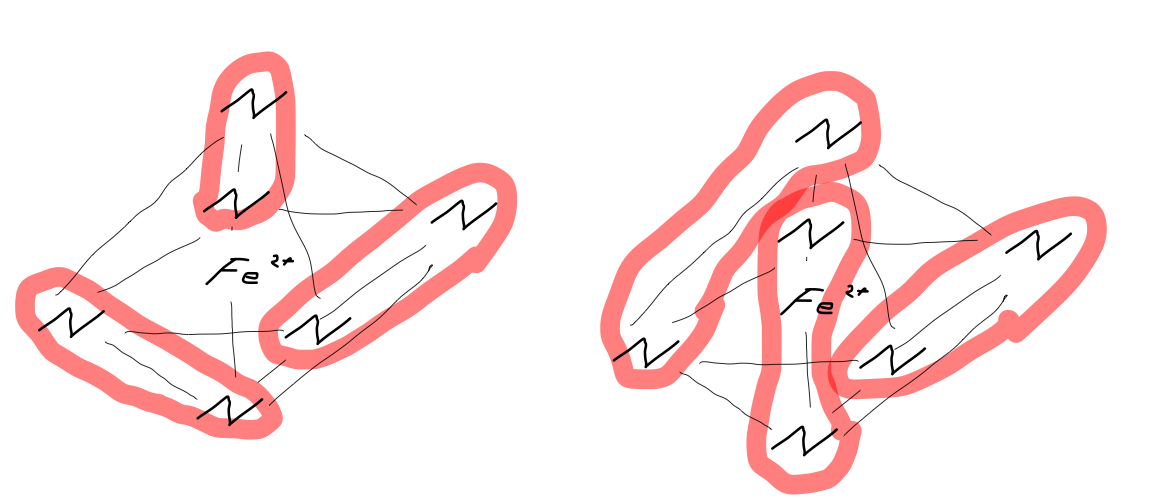
\includegraphics[clip, height=4cm]{imgs/phe-c.jpeg}
\caption{フェナントロリン}
\end{center}

\begin{center}
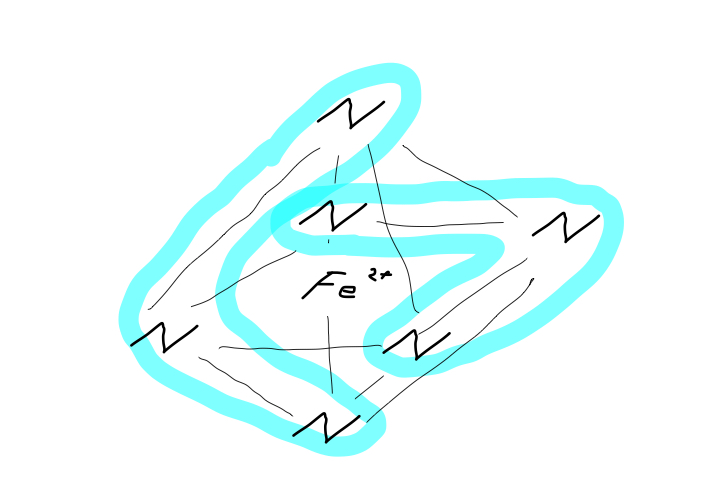
\includegraphics[clip, height=4cm]{imgs/ter-c.jpeg}
\caption{テルピリジン}
\end{center}
\end{figure}

\begin{tcolorbox}[colback=white,colbacktitle=black!10!white,coltitle=black,title={4}]
本実験では吸収極大を与える波長の吸光度を用いたが、それ以外の波長を用いても可能かどうか考察せよ。
\end{tcolorbox}

可能ではあるが、ノイズの影響を最も受けにくいのが吸収極大を与える波長であるので、なるべく吸収極大を与える波長で吸光度を測定した方が良い。

\subsection*{感想}
松枝さんへ

7thライブ幕張公演はday2のチケットが手に入りました。day1のチケットも頑張って手に入れたいと思います。

\newpage

\section*{実験 ll-2 蛍光法}
\begin{flushright}
実験日 : 2019/6/17

実習班 : 8班
\end{flushright}

\subsection*{目的}

蛍光スペクトルを測定する。

\subsection*{実験操作}
実習書にしたがって行った。

\subsection*{測定条件}
\subsubsection*{一般}
\begin{itemize}
\item 測定モード : 波長スキャン
\end{itemize}
\subsubsection*{装置}
\begin{itemize}
\item スキャンモード : 励起スペクトル or 蛍光スペクトル
\item データモード : 蛍光
\item (蛍光/励起)波長 : (蛍光/励起)スペクトルを見て入力
\item (励起/蛍光)開始波長 : 220 nm
\item (励起/蛍光)終了波長 : 700 nm
\item スキャンスピード : 300 nm/min
\item 初期待ち時間 : 0 sec
\item ホトマル電圧 : 400 V
\item レスポンス : 自動

\end{itemize}
\subsection*{結果(ピークの帰属を含む)}

スペクトルはレポート末に添付してあるのでそちらを参照。

\begin{table}[H]
\begin{center}
\begin{tabular}{|c|c|c|c|c|c|}
\hline
アセトニトリル希釈系列($\rm \mu M$) & 0.125 & 0.25   & 0.5    & 1     & 2      \\ \hline
系列1             & 63.56 & 119.6  & 242.3  & 508.9 & 1038   \\ \hline
系列2             & 57.9  & 118.7  & 253    & 542.9 & 1149   \\ \hline
平均              & 60.73 & 119.15 & 247.65 & 525.9 & 1093.5 \\ \hline
\end{tabular}
\caption{DNS-アラニンの検量線}
\end{center}
\end{table}

\pict{imgs/2-2-1.png}{8}

検量線の式をもとに未知試料の濃度を算出した結果402.5 $\rm  nM$となった。


\subsection*{考察}
未知試料の濃度は高めに出る傾向があるらしいが、実際の数値である400 nMとほとんど大きな差が出なかった。

\subsection*{課題}
\begin{tcolorbox}[colback=white,colbacktitle=black!10!white,coltitle=black,title={1}]
吸光法と蛍光法について、それぞれの長所と短所を比較してまとめよ。
\end{tcolorbox}

吸光法は蛍光を発さない物質にも適用できるので様々な物質に利用できるという利点があるが、励起光と透過光を同じ方向から見るためにノイズの影響を受けやすいという欠点がある。それに対して蛍光法は蛍光を発する物質にしか適用できないが、ノイズが小さいという利点がある。

\begin{tcolorbox}[colback=white,colbacktitle=black!10!white,coltitle=black,title={2}]
プリントの図をもとに、3つの蛍光スペクトルのうち1つが他と異なる理由を考察せよ。
\end{tcolorbox}

エチルアニリンとジメチルアニリンは基本的に脱プロトン化した状態が安定なため、脱プロトン化した状態での励起による蛍光しか観測されないが、ジエチルアニリンはプロトンがついた状態で存在する上に、その状態でも蛍光が観測されるため異なったスペクトルが現れる。


\subsection*{感想}
辛いです。

\newpage

\section*{実験 lll 蛍光顕微鏡法}
\begin{flushright}
実験日 : 2019/6/14

実習班 : 8班
\end{flushright}

\subsection*{課題}

\subsubsection*{1}
微小管の脱重合を阻害し、繊維を維持するため。

\subsubsection*{2}
\pict{imgs/kd3.jpeg}{8}

\subsubsection*{3}
\pict{imgs/kd4.jpeg}{10}
\subsubsection*{4}
\begin{table}[H]
\begin{center}
\begin{tabular}{|c|c|c|c|c|}
\hline
ATP濃度 [$\rm \mu M$] & 10 & 25 & 50 & 100 \\ \hline
キネシンの運動速度 [nm/s] & 439 & -       & 493          & 547    \\ \hline
\end{tabular}
\end{center}
\end{table}

\begin{enumerate}
\item [$\rm \mu M$]については動いているキネシンが存在しなかった。


\end{enumerate}
\subsubsection*{5}

10,50,100 $\rm \mu M$のキネシンの運動速度をL-Bプロットに代入した結果、$\rm V_{max} = 564 \ nm/s, \ K_m = 4.41 \  \mu M$となった。


\subsection*{感想}

研究室の中を色々見て回れたのが楽しかったです。

\end{document}